\documentclass{scu-thesis}
\usepackage{graphicx}	% for including graphics
% \usepackage{amsmath}	% for advanced typesetting of mathematics
% \usepackage{txfonts}	% for using the Times-Roman font
% \usepackage{natbib}	% for better citation styles
\usepackage[parfill]{parskip}

% These must be set first ... the rest of the thesis commands rely on them.

\author{Davis Allen}
\author{Robert Bayer}
\title{Conversation Station}
\department{Department of Computer Engineering}
\degree{Bachelor of Science in Computer Science and Engineering}

% Only bachelor's theses should have multiple authors and/or be from
% multiple departments.  Signatures required:
%
% Bachelor's theses: advisor(s), department chair(s)
% Master's theses: advisor, reader, department chair
% Doctoral theses: doctoral committee (including advisor), department chair

\begin{document}
\frontmatter
\signature{Thesis Advisor}
\signature{Thesis Advisor}f
\signature{Department Chair}
\signature{Department Chair}

\maketitle
\begin{abstract}
We are building a mobile application that will improve speed and personalization in conversations for people struggling with verbal communication. Many people diagnosed with Autism and other disorders face daily challenges involving communication due to speech impediments. Existing solutions allow users to communicate via speech cards or typing on a keyboard. However, these solutions make tradeoffs between personalization and speed, compromising what it takes to have fluid, natural, and rewarding conversations. Our solution will speed up personalized communication by applying machine learning principles. Our project will predict how a user will respond based on a combination of personal and collective language data, allowing the user to communicate quickly with their own voice.
\end{abstract}


\tableofcontents
\listoffigures

\mainmatter
\chapter{Introduction}

Communication is essential to building relationships. A person who has challenges speaking will face a lifetime of roadblocks in building friendships, connecting with family, and meeting daily needs. In the United States, it is estimated that 1 out of every 68 children will be diagnosed with some level of Autism\footnote[1]{Maguire, Corinne. "Autism on the Rise: A Global Perspective." Harvard College Global Health Review. (retrieved October 7, 2016).}, and many of these children will face communication challenges or be rendered completely nonverbal, depriving these children of a voice. As this number continues to rise\footnote[2]{Christensen, Deborah L.. "Prevalence and Characteristics of Autism Spectrum Disorder Among Children Aged 8 Years ? Autism and Developmental Disabilities Monitoring Network, 11 Sites, United States, 2012." Centers for Disease Control and Prevention. (retrieved October 7, 2016).}, finding ways for everyone to clearly communicate is essential to enhancing the human experience.

Today, nonverbal children such as those diagnosed with autism or Down syndrome communicate using many methods including gestures, sign language, and picture symbols. One of the most popular methods of communication is a device that generates speech. These devices come in many different forms. Some are similar to keyboards on which the child can type out what they want to say, while others have a list of buttons with pre-programmed messages from which the child can choose. Both of these options have also been incorporated into touchscreen devices such as the Apple iPad, so they are easily portable. 

While the ability to type out any response gives a flexible voice to the children, it can be tedious to retype similar responses and frustrating for all involved due to the time it takes to construct responses using a keyboard. The solutions with pre-programmed messages solve this problem by speeding up communication, but they impede the expressiveness of the children by limiting their response options. These limitations do not allow subtleties in diction, syntax, and personal preference to be communicated, erasing the voice from the personality behind it.

Using Machine Learning principles, Artificial Intelligence and Natural Language Processing, we developed an application that makes conversations quick but also personalized, giving people their own voice. We propose a solution that listens to conversations and gives the child several quick options to speak. These options will be personalized to each child, so that they maintain their voice. Additionally, we will have the option to type out a response if the available quick options are not what the child wants to communicate. The typed answers will be used to help the system learn how the child responds, thereby improving future suggestions. We plan on testing this solution with nonverbal children at Hope Technology School in Palo Alto, California.

Our solution combines the benefits of both current solutions, while eliminating the problems. By having the system learn about the child on an individual level, this communication tool will allow children to share their voice with the world. The inclusion of the quick suggestions will drastically improve response time, easing the communication process both between children and between verbal adults, such as the teacher or parent, and the child. Communication is crucial to forming human connections. Our proposed solution allows for seamless, fluid communication, giving everyone a voice.

\chapter{Requirements}

Listed below are the functional requirements, non-functional requirements, and design constraints of the project as gathered during the Requirements gathering phase. These requirements gave shape to our system and laid out what our system would become. The first category of requirements, functional requirements, details what our system will be able to do. Upon final evaluation, these requirements are either present or they are not, meaning that there is no middle ground and they are easily identifiable. The next category, non-functional requirements, describe how our system will behave. Unlike functional requirements, these requirements are not black-and-white and are evaluated on a qualitative rather than quantitative scale. This means that these requirements must be more closely evaluated and take into account the feedback from multiple perspectives, including the developer's and the user's perspective. Finally, the design constraints define the technological limitations that our system must adhere to. Design constraints limit the creative freedom the developers have to implement the system based on the constraints they must live within.

\section{Functional Requirements}
Critical:
\begin{itemize}
\item Provide input via the keyboard.
\item Capture audio via device microphone.
\item Speak through device speaker.
\item Suggest responses based on voice input.
\end{itemize}
Recommended:
\begin{itemize}
\item Provide input options via picture cards.
\end{itemize}
Suggested:
\begin{itemize}
\item Say keyword to activate microphone and save battery.
\end{itemize}

\section{Non-Functional Requirements}
Critical:
\begin{itemize}
\item The system will be able to handle multiple users.
\item The system's user interface will be intuitively designed.
\end{itemize}
Recommended:
\begin{itemize}
\item The system will be secure when storing private data.
\end{itemize}
Suggested:
\begin{itemize}
\item The system's user interface will be able to use graphics that are intuitive and familiar.
\item The system will be unaffected in loud environments.
\end{itemize}

\section{Design Constraints}
\begin{itemize}
\item The system must consist of a mobile application that runs on iPad devices.
\end{itemize}
\chapter{Use Cases}
\chapter{Activity Diagram}

The flowchart  outlines the workflow of all users? actions and interactions with the system. The diagram does not include the system actions, such as processing audible speech and displaying relevant suggestions.

\begin{figure}[htb]
\centering
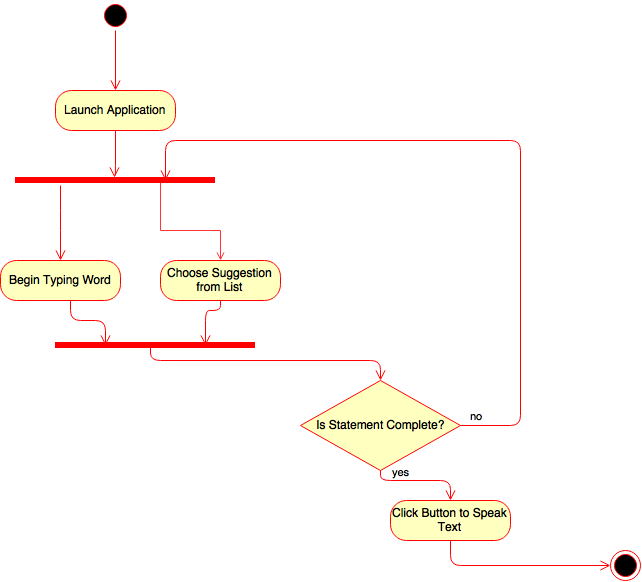
\includegraphics[width=\textwidth]{ActivityDiagram.png}
\caption{Mockup of text-entry user interface}
\label{fig:ui}
\end{figure}
\chapter{Conceptual Model}

Users will navigate to our application on an iPad tablet in order to use the system. Upon launching the app, they will be greeted with the keyboard view, as shown in Figure~\ref{fig:ui}, which they can immediately start using to type what they want to communicate.

\begin{figure}[htb]
\centering
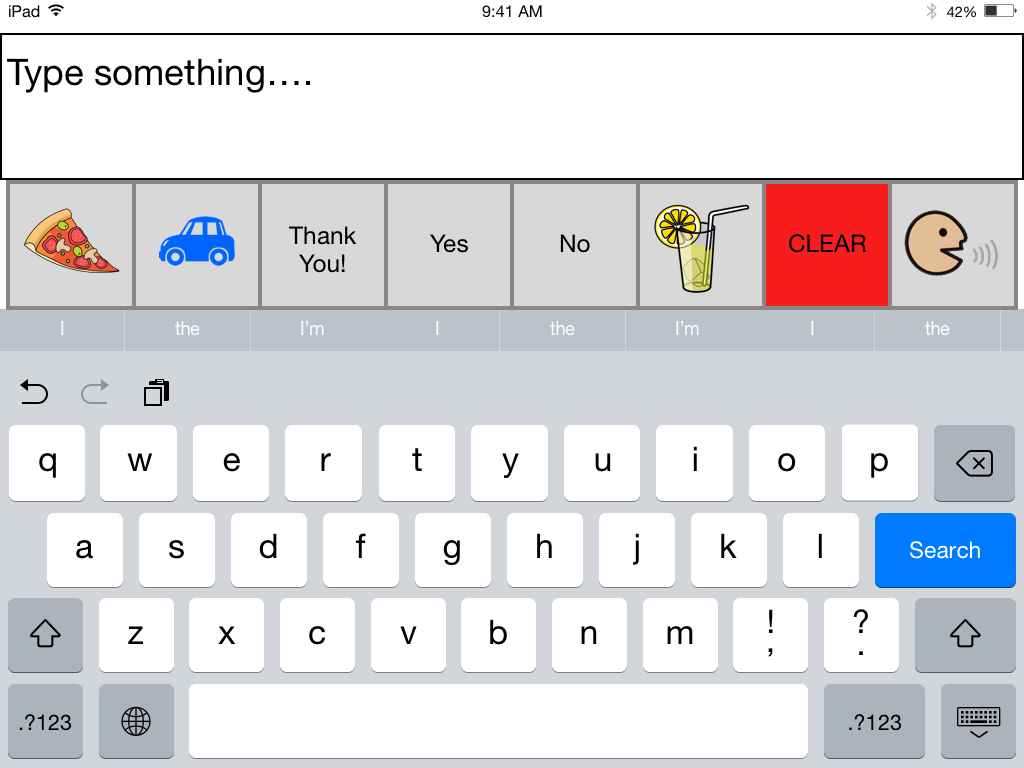
\includegraphics[width=\textwidth]{iPadLandscape.png}
\caption{Mockup of text-entry user interface}
\label{fig:ui}
\end{figure}

As they continue to type, the suggestions will adjust dynamically to both their input and any verbal feedback from the environment. The app will listen for audible speech, process the speech and prioritize the suggestions displayed to the user.  The system will first look for previous personal responses from the user to this or similar questions. After, it will display possible global responses from our database. In this way, previous personal responses will be prioritized above the global responses. This will be reflected in the application's interface as shown in Figure~\ref{fig:uiDynamic}.

\begin{figure}[htb]
\centering
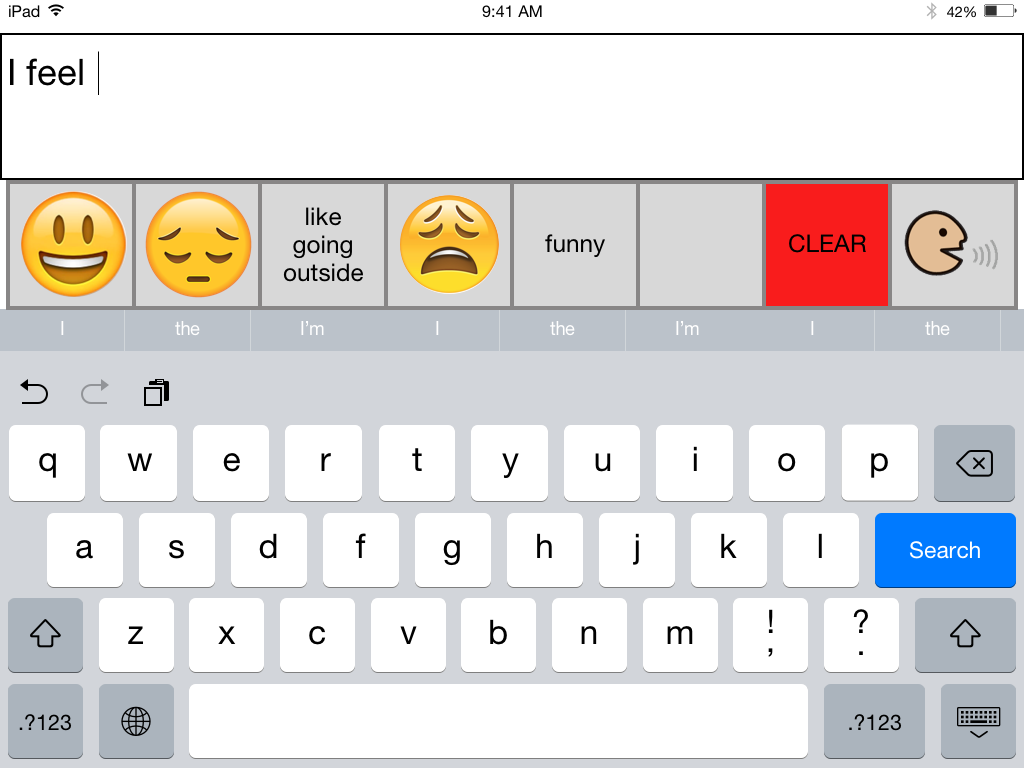
\includegraphics[width=\textwidth]{iPadLandscapeDynamic.png}
\caption{Mockup demonstrating the dynamic nature of suggestions}
\label{fig:uiDynamic}
\end{figure}

Whenever the user has completed either typing or selecting what they want to communicate, they will press the button on the right of the screen, which will speak what they have selected aloud. If the user then wants to clear the selection, they can use the clear button on the left of the speak button. This will allow the user to restart the process.

\chapter{Architectural Diagram}

We plan to utilize a basic client-server architecture to complete this project as shown in Figure~\ref{fig:arch}.

\begin{figure}[htb]
\centering
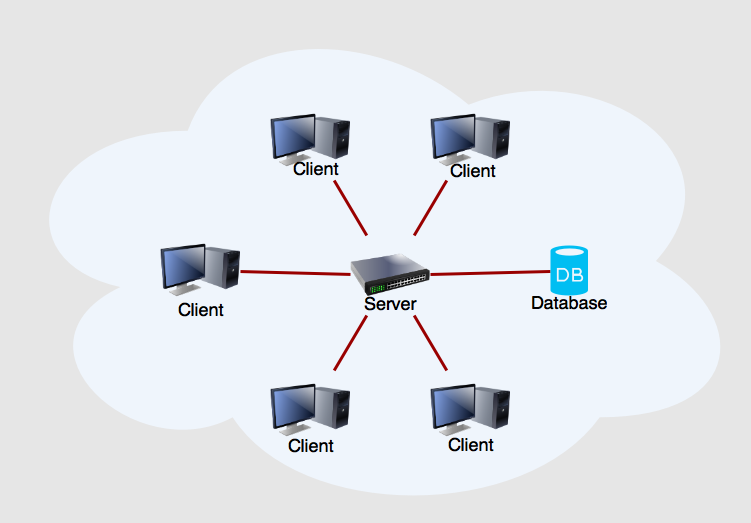
\includegraphics[width=\textwidth]{arch.png}
\caption{Client-Server Architecture}
\label{fig:arch}
\end{figure}

Users will be able to use our application on their mobile device, acting as a client, in order to access our site. The server in our system will be responsible for storing data for each child in the database, formulating a list of prioritized potential responses, and delivering these results to the client. The database will be relational, and the server will write to and read from it order to access data.
\chapter{Technologies Used}

\begin{itemize}
    \item Hardware
    \begin{itemize}
   	 \item Development
	 \begin{itemize}
   	 	\item Macbook Pro
		\item Macbook Air
	\end{itemize}
	 \item Application Testing
	  \begin{itemize}
   	 	\item iPads
		\item iPhones
	\end{itemize}
	 \item Server Processing
	  \begin{itemize}
   	 	\item Engineering Computing Center Servers
		\item Google App Engine
	\end{itemize}
    \end{itemize}
    \item Programming Languages
     \begin{itemize}
   	 	\item Swift
		 \begin{itemize}
   	 		\item For iOS Programming
		\end{itemize}
		\item Objective-C
		 \begin{itemize}
           	 	\item For iOS Programming
       	 	\end{itemize}
		\item Python
		 \begin{itemize}
   	 		\item For web server programming
		\end{itemize}
		\item JSON
		\begin{itemize}
   	 		\item For communicating with REST APIs
		\end{itemize}
	\end{itemize}
    \item IDEs
     \begin{itemize}
   	 	\item XCode
		\item MySQLWorkbench (or the like)
	\end{itemize}
    \item APIs
     \begin{itemize}
   	 	\item TensorFlow
		\item Cloud Natural Language API
		\item speech-to-text API
	\end{itemize}
    \item Database
     \begin{itemize}
   	 	\item Relational (depends on API integration)
		 \begin{itemize}
   	 		\item mySQL
			\item SQLite3
		\end{itemize}
	\end{itemize}
\end{itemize}
\chapter{Design Rationale}

We are leveraging a client-server model in order to minimize impact on the client mobile devices. In our model, a client will collect audial data and translate it into text to send to the server. The server will use NLP tools such as Google's Cloud Natural Language API to process the text and generate suggested responses to send back to the device as a JSON object. Having the server do the processing will minimize the use of the device's battery life, and will also decrease the disk space our app will require to be stored on the device. 

We are using iPads and other iOS devices for our testing because that is what our partners, the Hope Technology School, primarily uses in their classroom. This will eliminate the need for us to buy iPads for beta testers to use; saving money, time, and scheduling complexity.

Making use of the existing APIs like TensorFlow and Cloud Natural Language allows us to avoid re-inventing the wheel, and focus on how those tools can be used to fulfill our purpose. 

We will develop the application in XCode, using the Swift and Objective-C languages because they are the designated languages compatible with iOS to make applications. We will use Python to design the web server because we have experience using Google App Engine to make web servers specifically in Python and the APIs are well documented for the language.

Finally, we will use a relational database like SQLite and MySQL to store conversation data for the user. The data will be stored privately on the user's device and not in our servers because it is less vulnerable to attacks and will make minimal size impact in modern mobile devices.

\chapter{Testing Procedure}

Our testing process can be broken into three main sections: unit testing, an alpha release, and a beta release. Unit testing was done throughout the development process from Week 1 - 10 of Winter Quarter. Our alpha testing took place between Weeks 7 and 9 of Winter Quarter which was completed in participation with our industry expert at the Hope Technology School in Palo Alto, CA. At this point, the system was the first iteration of all the features of our application. The feedback from this stage helped us refine our interface and move into the beta, which took place from Weeks 1-5 of Spring Quarter.

\chapter{Risk Analysis}
\chapter{Ethical Analysis}

Even though our project can seem benevolent, there are several ethically ambiguous scenarios that must be considered and weighed prior to making decisions.


First, at an organizational level, our team has a couple of ethical dilemmas to consider. One such dilemma is how to ensure workload is being divided evenly among teammates. Like many problems, there seems to be a simple solution, by making a list of the work to be done and divide it evenly by number of tasks. But this process and judgment gets trickier with added complications, such as certain tasks requiring different amounts of time or team members missing deadlines. There are an infinite amount of potential situations to assess, so a global solution must be developed that can be applied across multiple scenarios. A good solution template would begin with a group discussion to try to work out the issue. If not everyone is satisfied with the results, we should schedule a meeting with our advisor to ask for him or her to mediate the discussion, allowing the experienced advisor to offer advice or make decisions for the team if necessary. Though this mediation strategy is generic it can be applied across multiple scenarios, which makes it a good basis for resolving ethical issues.


Secondly, concerning the social aspects of our project, there are many more ethical scenarios to consider in order to ensure that our application maximizes social benefits while minimizing concerns. One question we must consider is if we, as the developers, should have the power to control someone?s voice. Our application will try to predict what a user will typically say and how he or she would respond to a question. This gives us the capability to influence what options the user will choose in speaking. This feature can be potentially misused to influence and control someone?s voice in an extreme case. Questions determining the extent of control this application need to be evaluated to determine what kind of control the application should have in determining how a user will say something or respond to a question.


Thirdly, we have to consider the ethical implications of how our product system will be implemented. Our application will need to save records of the user?s conversations to remember the interests and voice patterns of the user. One situation to evaluate is the option to save that personal information locally on the user?s device or on our servers in the cloud. Both options have their respective pros and cons, namely that the cloud storage will improve speed and battery usage, and local storage will improve security. These trade-offs will force us to evaluate the situation and have us weigh the priority of features to determine how secure we need to store the user?s data. Likely, these priorities will be shifted as the application gets tested by users and they give feedback, so it will be important for our team to come back to this dilemma and re-evaluate the best storage option from time to time. The extent and implementation of features need to be evaluated and assessed in the development of our application with user safety in mind.


Conclusion Paragraph?

Notes from Google doc:
Bobby: I think we should include something in this section about developing a solution to a problem without the appropriate background (not dr.s or experienced in nonverbal communication techniques).
Davis: get lots of feedback and direction from the teacher and HTS. recognize that we are developers, not childhood development experts.


\include{developmentTimeline}
\chapter{Conclusion}

Over the course of this project we climbed over many walls to develop a consistent and finished product. This section contains results of how successful our design was, the lessons we learned along the way that helped develop our understanding and success in tackling large projects, and finally the future work we envision to build upon the project and create en even more robust and thorough solution.

\section{Results}
Our implemented design proved to be more effective at enabling quick and personalized conversation than other top solutions in the field. One way that our design improved the personalization of conversation was through our eight category response prediction algorithm. This algorithm sends the input statement to Google Cloud's Natural Language Processing API and receives a syntax and semantic breakdown of the statement. From this response, our algorithm determines which category of response is requested. For example, the question, "Where do you want to go for dinner?" will expect a "location" type response, and on the other hand the question "Who do you want to pick you up from school today?" will expect a "person" type response. Our system's ability to break down expected responses into eight different categories speeds up the user's ability to choose the right response they want to say and does not require them to make trade-offs in selecting an imperfect response to save time.

The next metric we used to classify the results of our system was a common metric in Human Computer Interaction (HCI) called the Number of Clicks metric. This simple metric measures the number of interactions a user must make with the app to perform the desired task. This is an important metric because speed is a huge factor in the success of a conversation, and therefore important to the success of our system. After our first meeting with our industry expert at the Hope Technology School, Christian Trifforiot confirmed that an average "click time" for a typical child with a nonverbal disability would take about six seconds, and that our application on average takes an average of 1.5 clicks to perform a desired operation \footnote{Trifforiot, Christian. (10 March 2017). Personal Interview}. Meaning that our application would take about nine seconds on average to formulate a response. Trifforiot also claimed that a leading competitor application called Proloquo2go \footnote{AssistiveWare. "Proloquo2go". Mobile Application. https://itunes.apple.com/us/app/ proloquo2go-symbol-based-aac/id308368164?mt=8} takes 7 clicks on average to perform a desired operation, meaning it can take up to 42 seconds to form a response. Our application is able to cut down response time to more than \(\frac{1}{3}\) of the response time by a leading application. This leads to a better user experience and improved conversation for the user and their converser.

\section{Lessons Learned}
Through much research, advice, and trial-and-error, we learned a lot of lessons that allowed us to deliver a completed project. We will continue to follow these principles and learn more as we take on any other projects and join other teams in the future.
\begin{enumerate}
	\item \textbf{Be wary of dependencies.} The more outside tools that your project relies on, the more points of failure are induced. Be careful  of using too many tools that are outside of your control, and be prepared for them to suddenly change or not work.
	\item \textbf{Multiply estimated time by 5.} In most circumstances, whatever time you estimate a task to take, it will take longer. Planning for unexpected development time will provide for a more accurate time assessment. 
	\item \textbf{Seek feedback early and often.} To avoid unexpected changes of requirements and unnecessary implementations of features that the customer may not want, maintain continuous contact with the customer. The earlier along in the development stages you can get feedback, the easier it is to iterate on those changes.
	\item \textbf{Build it up piece by piece.} Incremental design will allow for easy feature integration and natural divisions for unit testing. Building piece by piece will improve code understanding and reduce the number of unexpected errors.
\end{enumerate}

\section{Future Work}
Though our project demonstrated how using Natural Language Processing could be an invaluable tool in the application of predicting responses for people with nonverbal disabilities, there are many ways we see that our project could be improved. The following list details all the improvements we want to see developed to continue to help those 
\begin{enumerate}
	\item \textbf{Settings for voice options, number of displayed presets, and custom images in categories.}  There are many customization options we want to add to improve the app. We want to incorporate voice options for the user to select a male or female voice, because it is important for the user to really be able to identify the computer's voice as their own. For example, if a boy is using our application he may feel uncomfortable speaking with a female's voice, and vice versa. Next, we want to have a setting to adjust the number of displayed picture cards on the screen to raise or lower the complexity of decision-making for the user, depending on their age and level of ability. Finally, we want to provide an option to incorporate a user's own images in the picture card responses. For example, if a user gets prompted with the "Mom" response, it can be much more helpful for some children with mental disabilities to process a picture of their actual mother rather than a cartoon picture of a woman. Adding these options can significantly improve user experience and user retention for our application.
	\item \textbf{Improve question to answer mapping.} Our application talks to our server and receives feedback to predict what type of response is expected based on an input statement. Due to the limitations of Natural Language Processing, there are some cases where we cannot correctly predict what the user would actually say in response to a question. For example, if the input question reads, "What do you think of the Mona Lisa?", our application interprets Mona Lisa as a person, rather than a work of art. So, the user is presented with a person category rather than a work-of-art category. This is a small example that highlights the complexity of Natural Language Processing, but also shows us a road map for what developers and linguists can do to improve the tool and make it more universal and helpful for any situation.
	\item \textbf{Form sentences with suggested responses.} The current state of our application allows the user to choose a phrase or word in response to an input statement. We would like to expand this response into a completed sentence to improve conversation flow, truly giving the user their own uninhibited voice. For example, when the user is given the input statement of "What would you like to play with for recess?", the user can select from a list of items, and may say and answer like "basketball". Instead of giving a one-word answer, we would love to expand the response to something more like, "I would like to play basketball today," to make the conversation more realistic. This could improve the sociability of the user, teaching young children how to formulate sentences, and make it easier for the converser to understand the user's response.
	\item \textbf{Expand to other platforms.} Finally, we see lots of potential for how this system can be incorporated and integrated onto other platforms, especially wearable devices. The first step would be to make this available as an Android app so it is available on a lot more devices, especially to the majority of devices in third-world countries where Android devices are much more prevalent than iOS devices due to cost. Next, to allow this to be used on a smart watch or smart glasses like a pair of google glasses would allow the user the ability to converse through their device without needing to carry around an iPad everywhere they go. This would greatly increase the confidence and mobility of the user, also creating a more enjoyable user experience. The less invasive the technology is to the user's life and functions, the easier the system is able to integrate with anyone's lifestyle and circumstances.
\end{enumerate}

\chapter{User Manual}
\section{Installation}
\subsection{Server Setup}

None, the server is running at the URL hard-coded into the iOS mobile application. The server is already set up for you.

\subsection{iPad Application Installation}

\begin{enumerate}
\item Double click the Conversation Station.xcworkspace file to open it in Xcode.
\item Connect your iPad to the computer and select that iPad as the device to run the application.
\item Click Run from the menu to install the application and run it on the iPad.
\end{enumerate}

\section{Normal Use}
\begin{enumerate}
\item Install and launch the app.
\item Set the "wake" name, which should be the first name of the nonverbal child user.
\item Choose any option from the below list and repeat in a cycle until conversation is complete:
\begin{itemize}
\item Type a statement using the keyboard.
\item Speak the value of the input field over the iPad speakers.
\item Select a preset picture card to speak the associated word or phrase.
\item Select the listening button to trigger the device to begin processing verbal input.
\item Verbal user can say the nonverbal child user's "wake" name to trigger the device to begin processing verbal input.
\end{itemize}
\end{enumerate}
\chapter{Install Guide}
The development timelines shown in Figures~\ref{fig:fallQuarter},~\ref{fig:winterQuarter},~and~\ref{fig:springQuarter} below depict a set of tasks that need to be completed throughout the year. We used a Gantt Chart to break down our project into smaller deliverables. The horizontal blue lines split our work into three main sections: development, relationship, and documentation. We separated the larger chart into three individual charts, each corresponding to an individual academic school year.

\begin{figure}[htb]
\centering
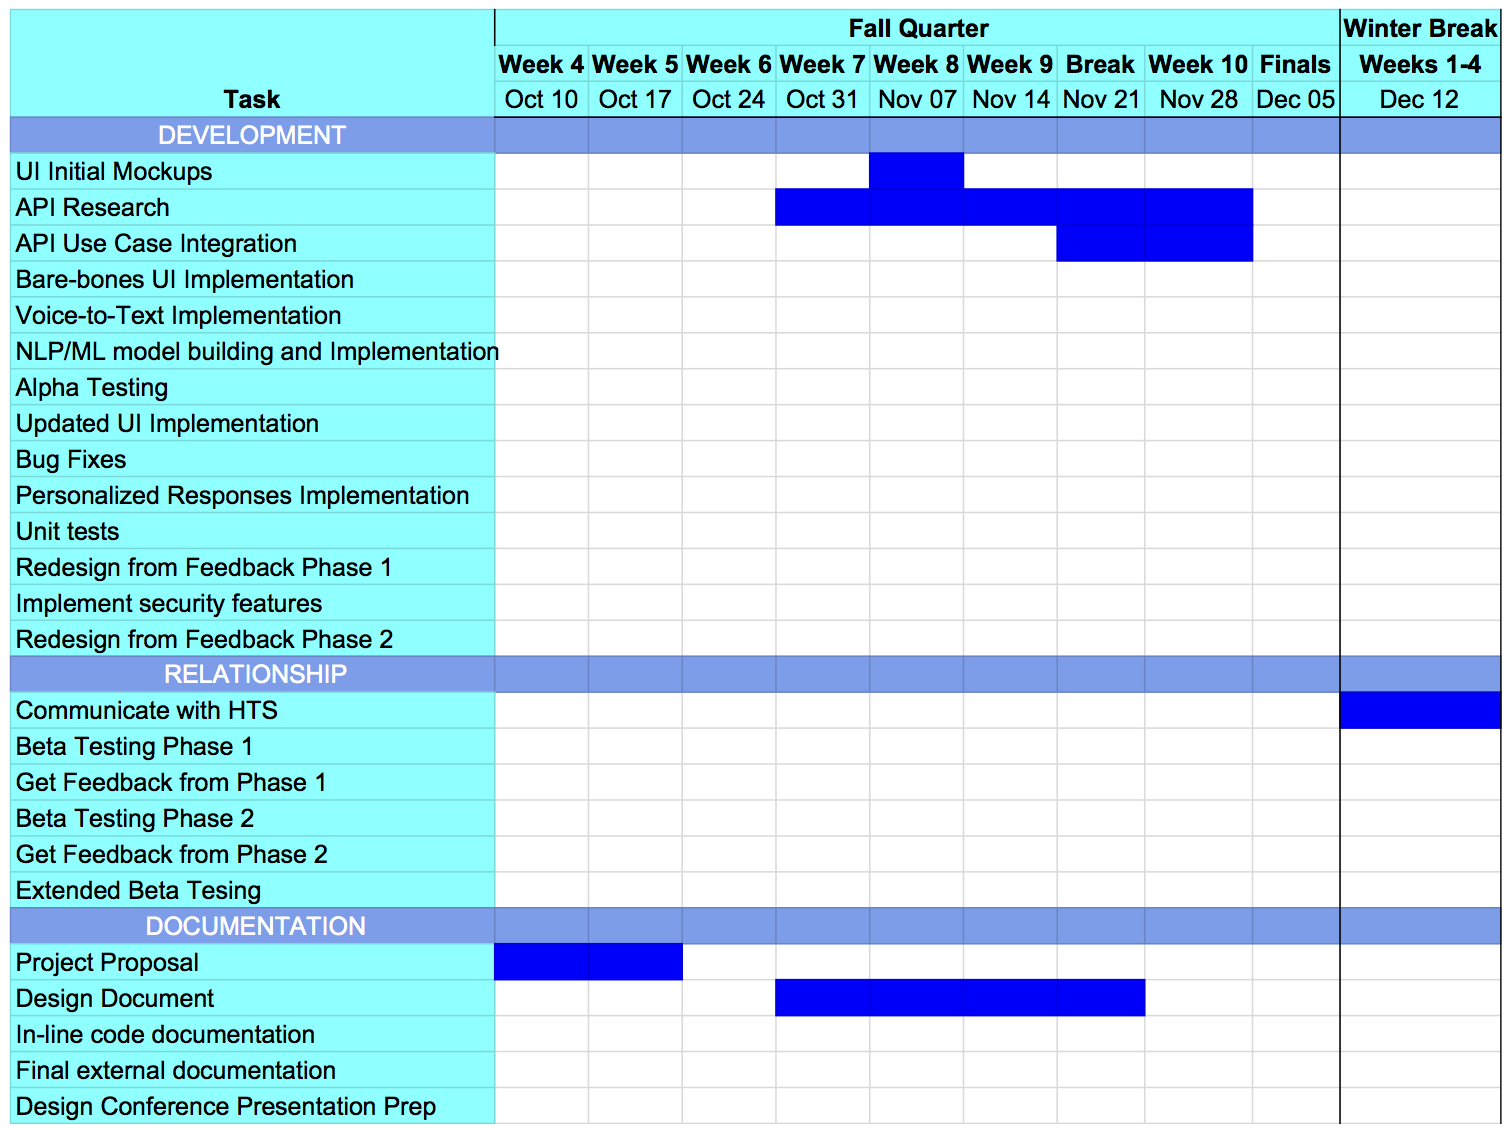
\includegraphics[width =\textwidth]{fallQuarter.png}
\caption{Fall Quarter Development Timeline Gantt Chart}
\label{fig:fallQuarter}
\end{figure}

\begin{figure}[htb]
\centering
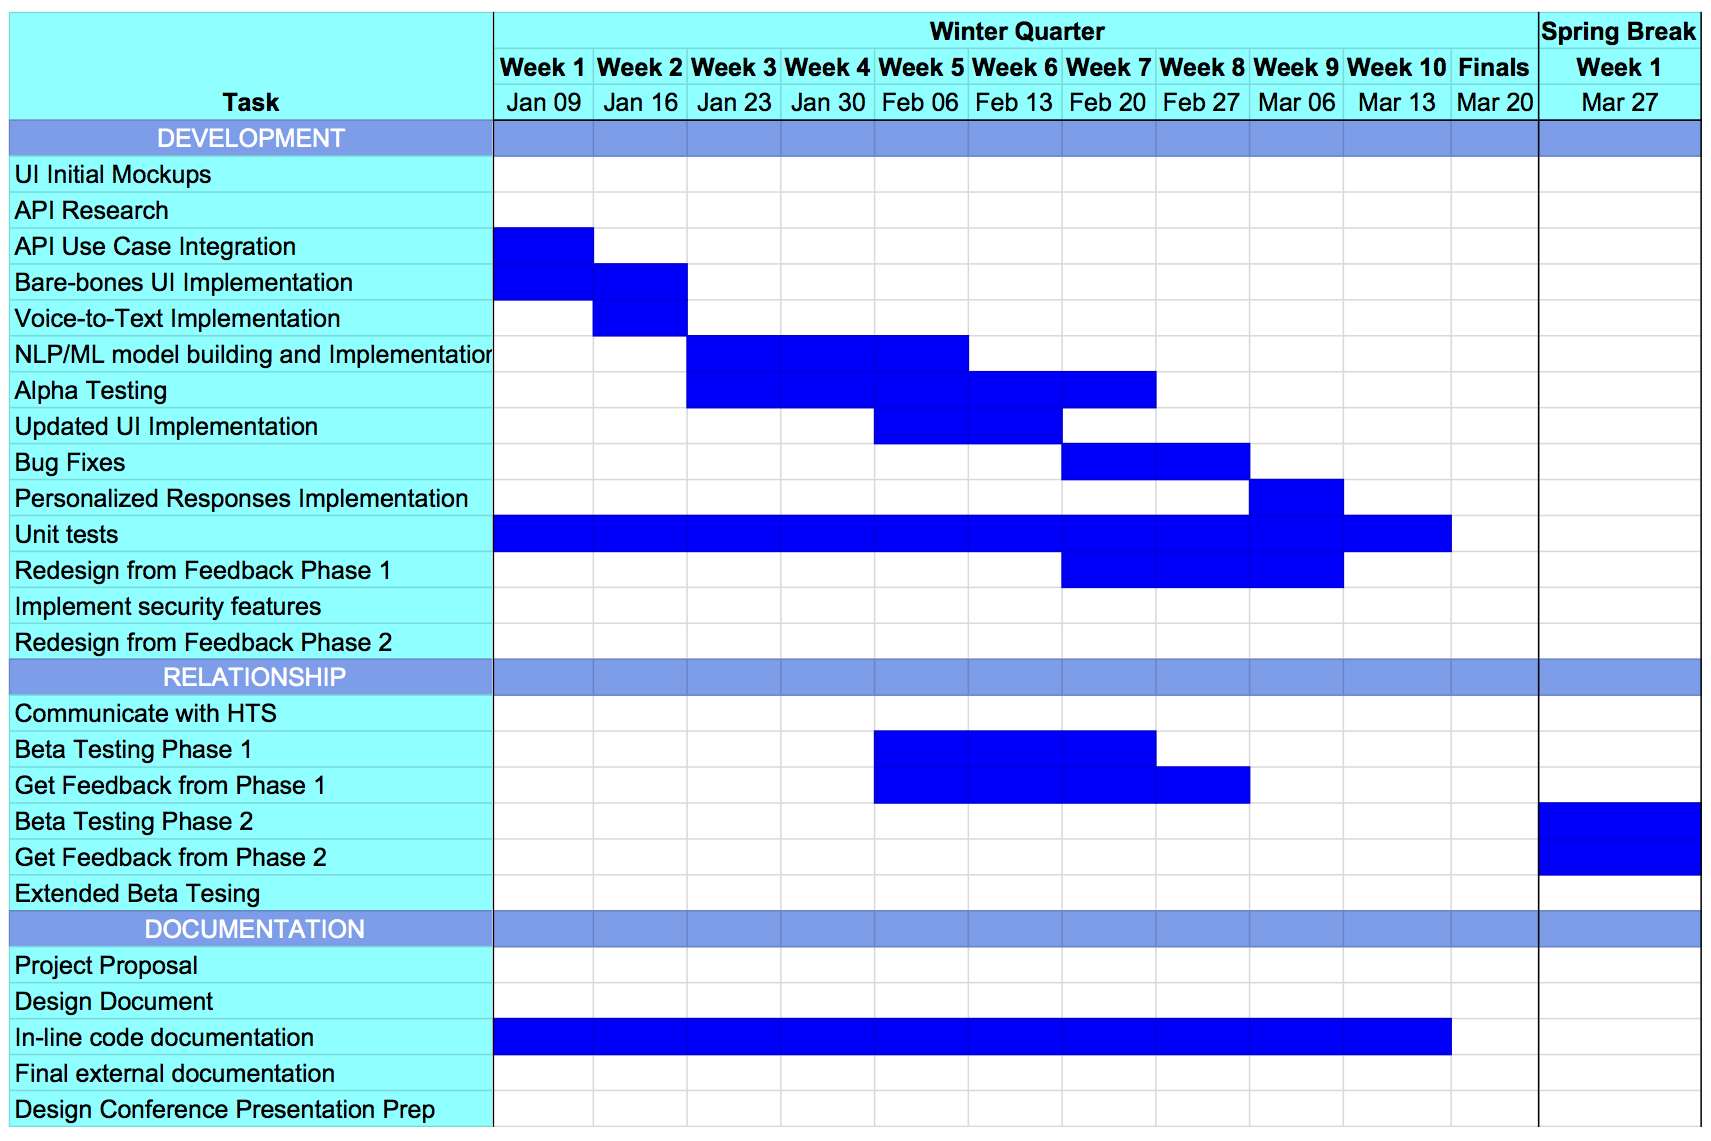
\includegraphics[width =\textwidth]{winterQuarter.png}
\caption{Winter Quarter Development Timeline Gantt Chart}
\label{fig:winterQuarter}
\end{figure}

\begin{figure}[htb]
\centering
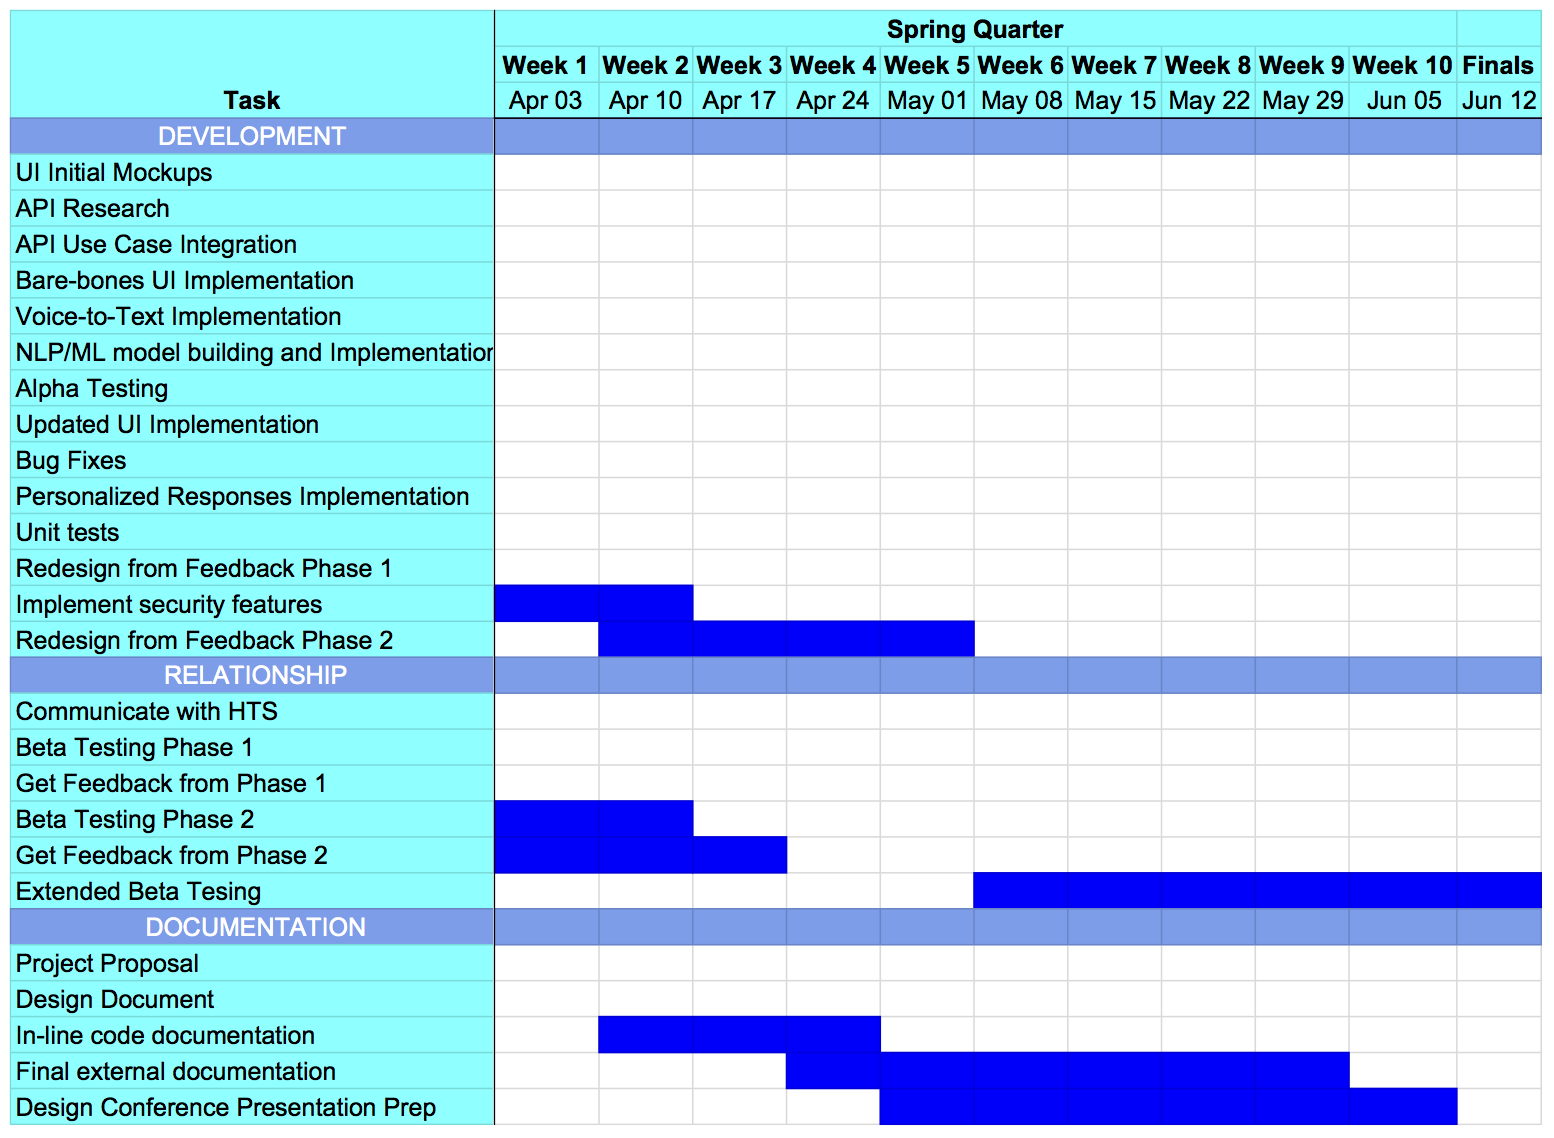
\includegraphics[width =\textwidth]{springQuarter.png}
\caption{Spring Quarter Development Timeline Gantt Chart}
\label{fig:springQuarter}
\end{figure}

\backmatter
\end{document}
